\documentclass[10pt,a4paper]{article}
\usepackage[top=1.36in, bottom=1.36in, left=0.98in, right=0.98in]{geometry}
\usepackage[utf8]{inputenc}
\usepackage[czech]{babel}
\usepackage{tikz}
\usepackage{pgfplots}
\usepackage{xcolor,listings}
\usepackage{textcomp}
\usepackage{hyperref}
\usepackage{graphicx}
\usepackage{amsmath}
\usepackage{algorithm}
\usepackage{listings}
\usepackage{fontspec,minted}
\usepackage{subfig}
\usepackage{xevlna}

\title{Analýza obrazu II//Detekce parkovacích míst}
\author{Richard Zvonek}


\definecolor{backcolour}{rgb}{0.1686,0.1686,0.1686}

\newminted{c++}{
  style=monokai,,
  bgcolor=backcolour,
  fontsize=\small,
  frame=lines
}

\setmonofont{[JetBrainsMono-Regular.ttf]}[Contextuals=Alternate,Ligatures=TeX]


\begin{document}

\begin{center}
  {\Large Vysoká Škola Báňská – Technická Univerzita Ostrava\par
    Fakulta Elektrotechniky a Informatiky\par
    Katedra Informatiky\par}
  \vspace{26mm}
  {\Huge\bfseries Analýza obrazu II \par}
  \bigskip
  {\Huge\bfseries Detekce obsazenosti parkovacích míst \par}
\end{center}
\vfill
{\Large\number\year\hfill Richard Zvonek, ZVO0016}
\cleardoublepage

\newpage

\tableofcontents

\newpage

\section{Zadání}
Na zadaných testovacích datech detekovat obsazenost parkovacích míst, vyzkoušet metody s trénováním, bez trénování a srovnat výsledky. Pro srovnání výsledků vypsat počet nesprávně určených (false positive, false negative) výsledků a F1 score.\par
Testovací sada obsahuje 24 fotografií parkovacích míst, obsahující různě zaplněné parkoviště v různé denní doby.

\begin{figure}[ht]%
  \centering
  \subfloat[Testovací obraz]{{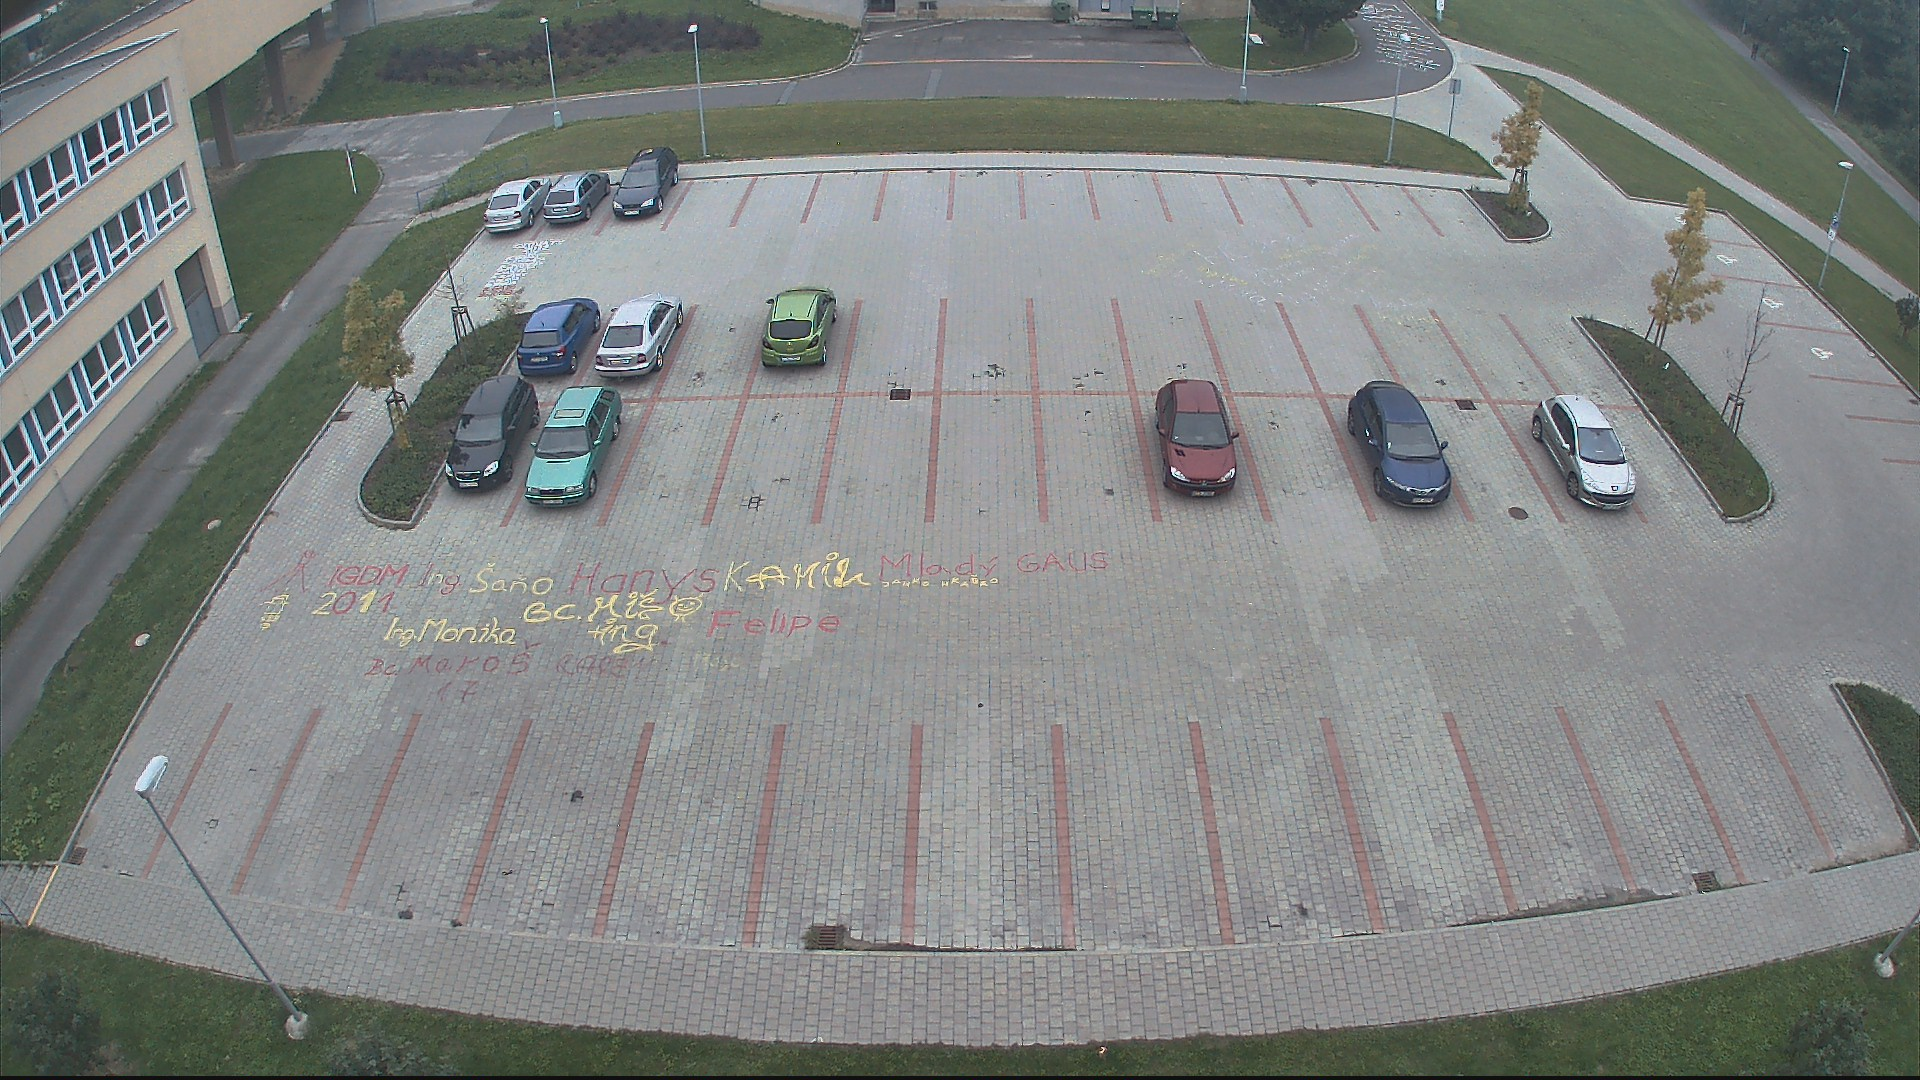
\includegraphics[width=10cm]{images/test10.jpg} }}%
  \qquad
  \subfloat[Noční testovací obraz]{{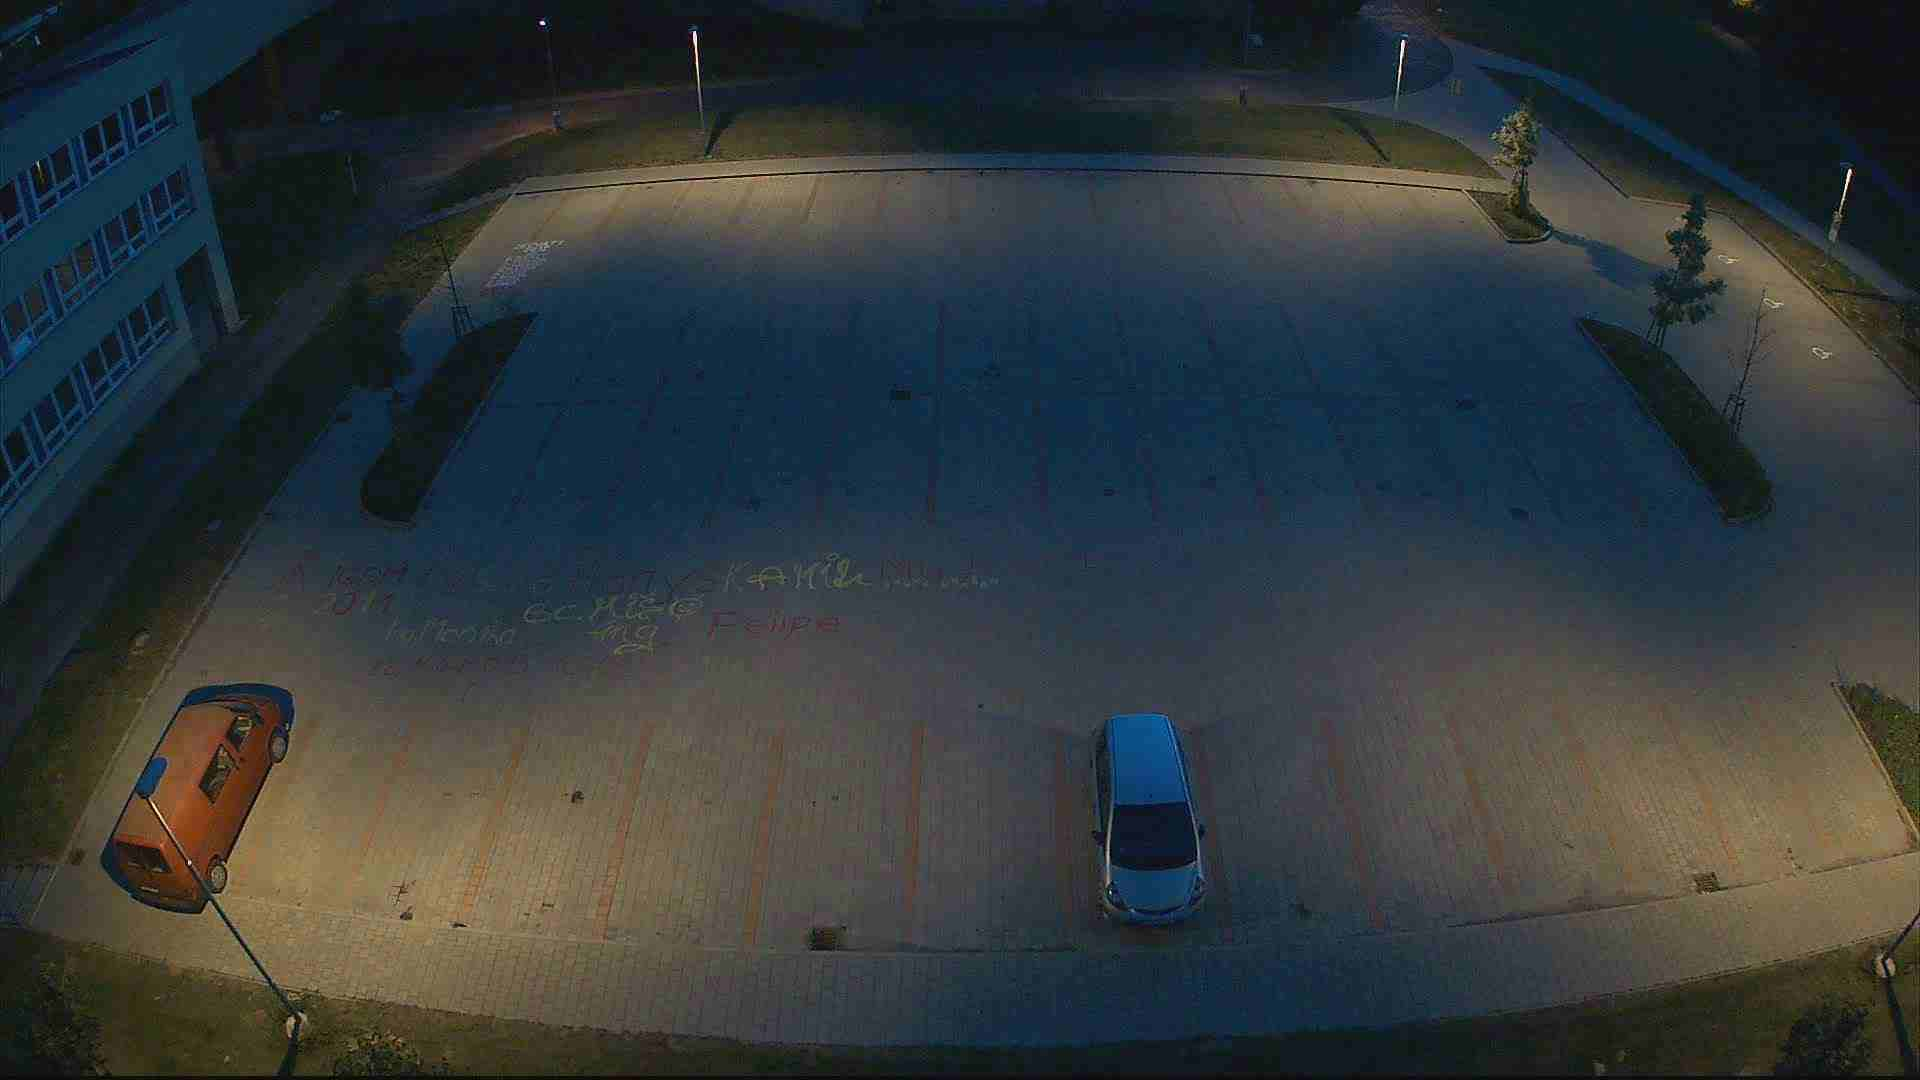
\includegraphics[width=10cm]{images/test15.jpg} }}%
  \qquad

  \caption{Ukázka testovacích obrazů}%
  \label{fig:testData}%
\end{figure}

\section{Detekce bez trénování}
\section{Detekce s trénováním}
\subsection{Trénovací data}
Pro trénování neuronových sítí byly dodány trénovací obrazy prázdných a plných parkovacích míst. Nevýhodou dodaných trénovacích dat je absence nočních snímků. Na tento nedostatek neuronové sítě trpěly, proto jsem se rozhodl implementovat umělé rozšíření datové sady. Pro výpočet rozšíření datové sady jsem využil vysoce sofistikovaného postupu, viz \hyperref[lst:extendedImagesAlgo]{výpis \ref{lst:extendedImagesAlgo}}. Po rozšíření trénovací sady se celkový počet trénovacích dat zosminásobil, ukázka výsledku rozšíření je zobrazen na \hyperref[fig:testData]{obrázcích \ref{fig:testData}}. \par
Po aplikaci rozšíření se zvýší doba trénování neuronové sítě, zvýší se paměťová náročnost GPU při tréninku, ale celková přesnost se podstatně zvýší (v řádu jednotek procent).

\begin{listing}[ht]
\begin{c++code}
void TrainInputSet::getExtendedImages(const cv::Mat &inputImg,
std::vector<cv::Mat> &extendedImages) {
    cv::Mat flippedx;
    cv::Mat flippedy;
    cv::Mat flippedxy;

    cv::flip(inputImg, flippedx, 0);
    cv::flip(inputImg, flippedy, 1);
    cv::flip(inputImg, flippedxy, -1);

    extendedImages.emplace_back(flippedx);
    extendedImages.emplace_back(flippedy);
    extendedImages.emplace_back(flippedxy);

    // Simulate night
    extendedImages.emplace_back(inputImg / 2);
    extendedImages.emplace_back(flippedx / 3);
    extendedImages.emplace_back(flippedy / 4);
    extendedImages.emplace_back(flippedxy / 5);
  }
\end{c++code}
\caption{Výpočet rozšíření datové sady}
\label{lst:extendedImagesAlgo}
\end{listing}

\subsection{Použité neuronové sítě}

\subsubsection{LeNet}
\paragraph{Architektura sítě}
\subsubsection{AlexNet}
\paragraph{Architektura sítě}


\subsection{Srovnání}

\clearpage
\section*{Přílohy}


\subsection*{Srovnání neuronových sítí}
\begin{table}[]
  \begin{tabular}{r|lllllll}
    DNN                       &
    \begin{tabular}[c]{@{}l@{}}Velikost \\ obrazu\end{tabular} &
    \begin{tabular}[c]{@{}l@{}}Learning \\ Rate\end{tabular} &
    \begin{tabular}[c]{@{}l@{}}Min \\ Learning \\ Rate\end{tabular} &
    \begin{tabular}[c]{@{}l@{}}Batch \\ size\end{tabular} &
    \begin{tabular}[c]{@{}l@{}}Max steps \\ without progress\end{tabular} &
    \begin{tabular}[c]{@{}l@{}}Max \\ epochs\end{tabular} &
    \begin{tabular}[c]{@{}l@{}}Doba \\ tréninku\end{tabular}   \\
    \hline
    LeNet                     &
    $28 \times 28$            &
    $0.01$                    &
    $10^{-6}$                 &
    $128$                     &
    $1000$                    &
    $300$                     &
    $\approx 45s$\footnotemark  \\

    AlexNet                   &
    $80 \times 80$            &
    $0.01$                    &
    $0.001$                   &
    $256$                     &
    $1000$                    &
    $300$                     &
    $800s \sim 1000s$           \\

    Vgg19                     &
    $32 \times 32$            &
    $0.01$                    &
    $10^{-7}$                 &
    $64$                      &
    $500$                     &
    $300$                     &
    $\approx 3000s$             \\

    ResNet                    &
    $32 \times 32$            &
    $0.01$                    &
    $10^{-7}$                 &
    $64$                      &
    $128$                     &
    $300$                     &
    $\approx 40s$               \\

    GoogLeNet                 &
    $32 \times 32$            &
    $0.01$                    &
    $10^{-7}$                 &
    $64$                      &
    $128$                     &
    $300$                     &
    $\approx 35s$               \\\hline \\
  \end{tabular}
  \caption{Nastavení neuronových sítí}
  \label{tab:dnnSetting}
\end{table}


\footnotetext{Trénování a rozpoznávání bylo testováno na Manjaro Linux x86\_64 5.8.18, Intel i5-5200U@2.7GHz, NVIDIA GeForce GTX 850M, 4GB VRAM}

\begin{table}[]
  \begin{tabular}{r|lllllll}
    DNN                        &
    \begin{tabular}[c]{@{}l@{}}False \\ positives\end{tabular} &
    \begin{tabular}[c]{@{}l@{}}False \\ negatives\end{tabular} &
    \begin{tabular}[c]{@{}l@{}}Přesnost \\ rozpoznání \\ Rate\end{tabular} &
    \begin{tabular}[c]{@{}l@{}}F1 \\ score\end{tabular}   \\
    \hline
    LeNet                      &
    $28 \times 28$             &
    $0.01$                     &
    $10^{-6}$                  &
    $128$                        \\

    AlexNet                    &
    $80 \times 80$             &
    $0.01$                     &
    $10^{-6}$                  &
    $128$                        \\

    Vgg19                      &
    $32 \times 32$             &
    $0.01$                     &
    $10^{-7}$                  &
    $128$                        \\

    ResNet                     &
    $32 \times 32$             &
    $0.01$                     &
    $10^{-7}$                  &
    $128$                        \\\hline \\
  \end{tabular}
  \caption{Výsledky neuronových sítí}
  \label{tab:dnnResults}
\end{table}


\subsection*{Rozšířená trénovací sada}
\newcommand\testImgWitdth{4cm}

\begin{figure}[ht]%
  \centering
  \subfloat[Originál]{{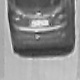
\includegraphics[width=\testImgWitdth]{images/1000_orig.jpg} }}%
  \qquad
  \subfloat[Překlopený obraz podle x]{{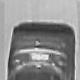
\includegraphics[width=\testImgWitdth]{images/1000flipx.jpg} }}%
  \qquad
  \subfloat[Překlopený obraz podle y]{{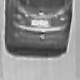
\includegraphics[width=\testImgWitdth]{images/1000flipy.jpg} }}%
  \qquad
  \subfloat[Překlopený obraz podle xy]{{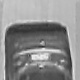
\includegraphics[width=\testImgWitdth]{images/1000flipxy.jpg} }}%
  \qquad
  \subfloat[Noční obraz s jasem $\frac{1}{2}$]{{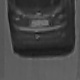
\includegraphics[width=\testImgWitdth]{images/1000_orig_night.jpg} }}%
  \qquad
  \subfloat[Noční obraz s jasem $\frac{1}{3}$]{{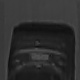
\includegraphics[width=\testImgWitdth]{images/1000flipx_night.jpg} }}%
  \qquad
  \subfloat[Noční obraz s jasem $\frac{1}{4}$]{{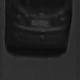
\includegraphics[width=\testImgWitdth]{images/1000flipy_night.jpg} }}%
  \qquad
  \subfloat[Noční obraz s jasem $\frac{1}{5}$]{{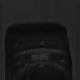
\includegraphics[width=\testImgWitdth]{images/1000flipxy_night.jpg} }}%
  \qquad

  \caption{Ukázka rozšířené trénovací sady}%
  \label{fig:testData}%
\end{figure}

\end{document}
